\chapter{Design}

\section{Overall System Design}

\subsection{Short description of the main parts of the system}

\subsection{System flowcharts showing an overview of the complete system}

\section{User Interface Designs}

\section{Program Structure}

\subsection{Top-down design structure charts}

\subsection{Algorithms in pseudo-code for each data transformation process}

\subsection{Object Diagrams}

\subsection{Class Definitions}

\section{Prototyping}

\section{Definition of Data Requirements}

\subsection{Identification of all data input items}

\subsection{Identification of all data output items}

\subsection{Explanation of how data output items are generated}

\subsection{Data Dictionary}

\begin{tabular}{|p{1.5cm}|p{1.5cm}|l|l|l|p{2.5cm}|}
	\hline
	NAME & DATA TYPE & LENGTH & VALIDATION & EXAMPLE DATA & APPROXIMATE SIZE \\ \hline
	Name & String & 1 - 100 Characters & Length & Peter Millard & 100 Bytes \\ \hline
	Position & Integer & 1 - 50 & Range & 05 & 4 Bytes \\ \hline
	Watch Time & Time & 00:15:00 - 02:00:00 & Range & 01:10:23 & 3 Bytes \\ \hline
	Club & String & 1 - 100 Characters & Range & Team Cambridge &  100 Bytes\\ \hline
	Date & date & DD/MM/YYYY & Length & 17/10/1995 & 3 Bytes \\ \hline
	Ride Time & Time & 00:15:00 - 02:00:00 & Range & 00:24:43 & 3 Bytes \\ \hline
	Handicap Time & Time & 0:00 - 31:44 & Range & 16:59 & 3 Bytes \\ \hline
	Handicap Points & Integer & 0 - 350 & Range & 176 & 4 Bytes \\ \hline
	Handicap Position & Integer & 1 -100 & Range & 5 & 4 Bytes \\ \hline
	Transmedia Points & Integer & 0- 350 & Range & 190& 4 Bytes \\ \hline
	Circuit Points & Integer & 0 - 200 & Range & 72 & 4 Bytes \\ \hline	
	Juvenile Points & Integer & 0 - 350 & Range & 30 & 4 Bytes \\ \hline
	Hill Climb Points & Integer & 0 - 100 & Range & 20 &  4 Bytes\\ \hline
\end{tabular}

\subsection{Identification of appropriate storage media}

\section{Database Design}

\subsection{Normalisation}

\subsubsection{ER Diagrams}
\begin{figure}[H]
    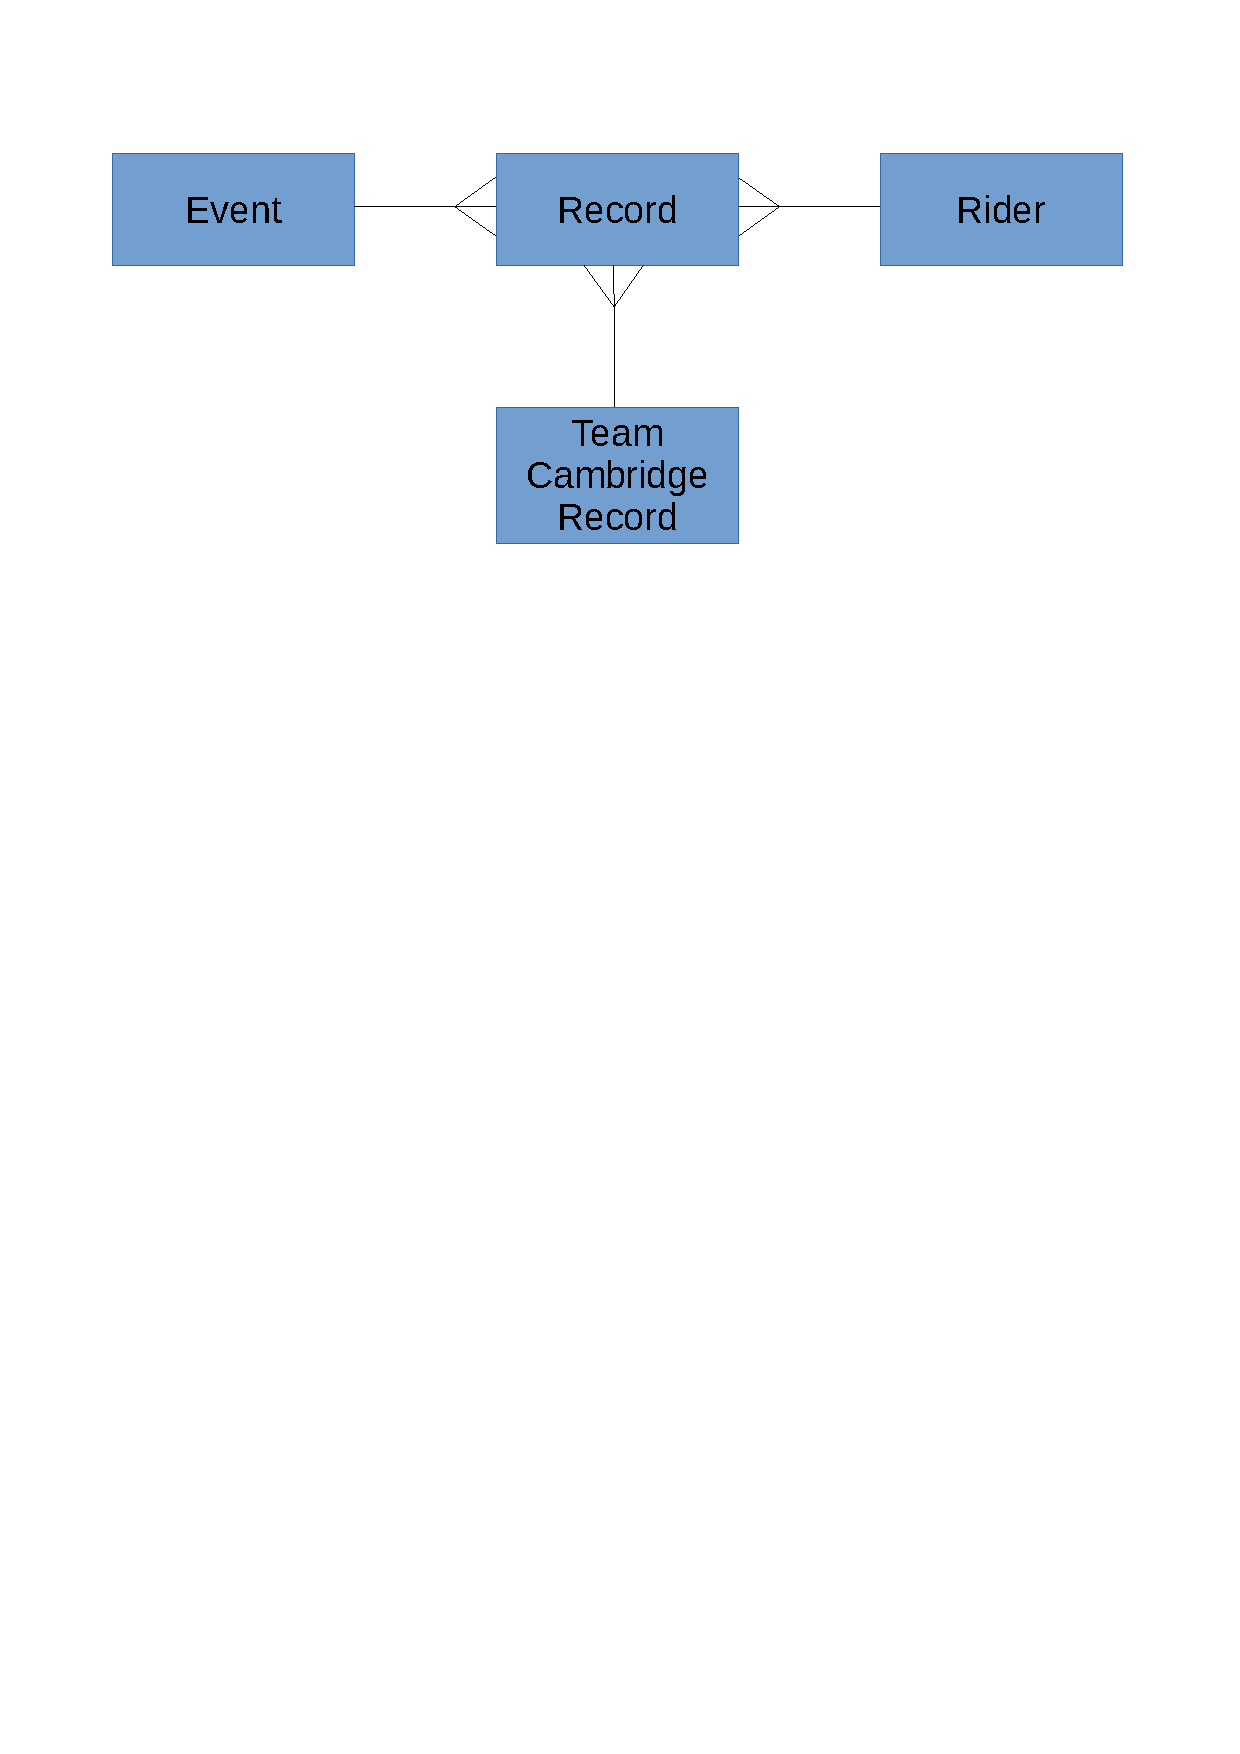
\includegraphics[width=\textwidth]{./ER/ERDesing.pdf}
\end{figure}

\subsubsection{Entity Descriptions}
After looking the specification, I found that there was attributes missing from the entity that needed to be included so I modified the entity descriptions from the analysis.

<<<<<<< HEAD
Event(\underline{EventID}, \emph{CourseID}, Date, Handicap10, Handicap25, HillClimb, Transmedia, Circuit Series, Juvenile, Code)
=======
Event(\underline{EventID}, \emph{CourseID}, Date, CircuitSeries, Handicap10, Handicap25, HillClimb, Transmedia, Juvenile, Code)
>>>>>>> branch 'master' of https://github.com/24697/COMP4Coursework.git

Rider(\underline{RiderID}, Forename, Surname)

<<<<<<< HEAD
TeamCambridgerecord(\underline{TCID},\emph{RecordID}, HandicapPoints, TransmediaPoints,CircuitPoints, JuvenlePoints)
=======
TCRecord(\underline{TCID},\emph{RecordID}, Handicap10Points, CircuitPoints, TransmediaPoints, JuvenlePoints)
>>>>>>> branch 'master' of https://github.com/24697/COMP4Coursework.git

Course(\underline{CourseID}, EventCode)

Record(\underline{RecordID}, \emph{RiderID},\emph{EventID}, RideTime, HandicapTime, RacePosition, Club, Age)

\subsubsection{1NF to 3NF}

\subsubsubsection{UNF}

\begin{itemize}
\item \underline{EventID}
\item \emph{CourseID}
\item Date
\item CircuitSeries
\item Handicap10
\item Handicap25
\item HillClimb
\item Transmedia
\item Juvenile
\item Code
\item \underline{RiderID}
\item Forename
\item Surname
\item \underline{TCID}
\item Handicap10Points
\item CircuitPoints
\item TransmediaPoints
\item JuvenlePoints
\item \underline{CourseID}
\item EventCode
\item \underline{RecordID}
\item RideTime
\item HandicapTime
\item RacePosition
\item Club
\item Age
\end{itemize}

\subsubsubsection{UNF to 1NF}

\begin{tabular}{|l|l|}
\hline
REPEATING & NON-REPEATING \hline
\underline{RiderID} & \underline{EventID} \hline
\emph{EventID} & Date \hline
Forname & CircuitSeries \hline 
Surname & Handicap10 \hline 
TCID & Handicap25 \hline
Handicap10Points & HillClimb \hline 
CircuitPoints & Transmedia \hline
TransmediaPoints & Juvenile \hline
JuvenilePoints & Code \hline
RecordID & CourseID \hline
RideTime & EventCode \hline
HandicapTime & \hline
RacePosition & \hline
Club & \hline
Age & \hline

\end{tabular}

\subsubsubsection{1NF to 2NF}



\subsubsubsection{2NF to 3NF}



\section{Security and Integrity of the System and Data}

\subsection{Security and Integrity of Data}

\subsection{System Security}

\section{Validation}

\section{Testing}

\begin{landscape}
\subsection{Outline Plan}

\begin{center}
    \begin{tabular}{|p{2cm}|p{5cm}|p{5cm}|p{4cm}|}
        \hline
        \textbf{Test Series} & \textbf{Purpose of Test Series} & \textbf{Testing Strategy} & \textbf{Strategy Rationale}\\ \hline
        Example & Example & Example & Example \\ \hline
    \end{tabular}
\end{center}

\subsection{Detailed Plan}

\begin{center}
    \begin{longtable}{|p{1.5cm}|p{2.5cm}|p{2.5cm}|p{2cm}|p{2cm}|p{2cm}|p{2cm}|p{2cm}|}
        \hline
        \textbf{Test Series} & \textbf{Purpose of Test} & \textbf{Test Description} & \textbf{Test Data} & \textbf{Test Data Type (Normal/ Erroneous/ Boundary)} & \textbf{Expected Result} & \textbf{Actual Result} & \textbf{Evidence}\\ \hline
        Example & Example & Example & Example & Example & Example & Example & Example \\ \hline
    \end{longtable}
\end{center}
\end{landscape}
